% Asset ID: AS1TrigonometricRatiosTIKZ-009
% Source: P1-Chp9 pp.23-24
% Related section: Sine Rule Twice
% Purpose: Triangle requiring sine rule twice
\documentclass[tikz,border=8pt]{standalone}
\usepackage{amsmath}
\usetikzlibrary{angles,quotes,calc,arrows.meta}
\begin{document}
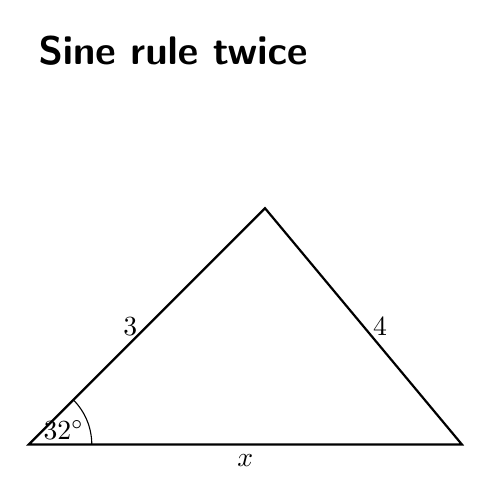
\begin{tikzpicture}[scale=1.0, every node/.style={font=\sffamily}]
\node[font=\sffamily\bfseries\Large, anchor=west] at (0,5) {Sine rule twice};
\coordinate (A) at (0,0);\coordinate (B) at (5.5,0);\coordinate (C) at (3,3);\draw[thick] (A)--(B)--(C)--cycle;\node[below] at ($(A)!0.5!(B)$) {$x$};\node[right] at ($(B)!0.5!(C)$) {$4$};\node[left] at ($(A)!0.5!(C)$) {$3$};\pic[draw,"$32^\circ$",angle radius=.8cm] {angle=B--A--C};
\end{tikzpicture}
\end{document}
